\section{Simulations and Results}\label{sec:04:results}
All analog simulations are performed in the language of \textit{AIMSpice} in the \textit{AIM-Spice} computer program. All digital simulations are performed in the language \textit{Verilog}, with the editor \textit{VSCode}, compiler \textit{Icarus Verilog} and waveform plotter \textit{gtkwave}. All code used to simulate can be found in the appendix.

\subsection{Analog bitcell}
The analog behavior of the bitcell is simulated to show the functionality at different temperatures and with different configurations of slow/fast nmos/pmos transistors, as well as the read-time, the write-time and the leakage current for the SS, TT and FF configurations.

\subsubsection{Leakage current}
The leakage currents at different configurations are shown in \autoref{fig:04:leakage}. The current is negative, so keep in mind that it is the absolute value of the current which is of interest. It would ideally be as close to zero as possible to keep power consumption down.

\begin{figure}[H]
    \centering
    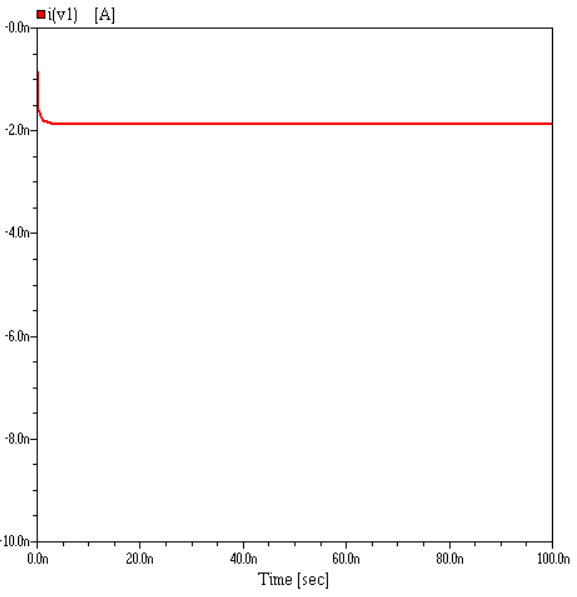
\includegraphics[width=0.3\linewidth]{aimSpice/plots/plotsSS/leak.png}
    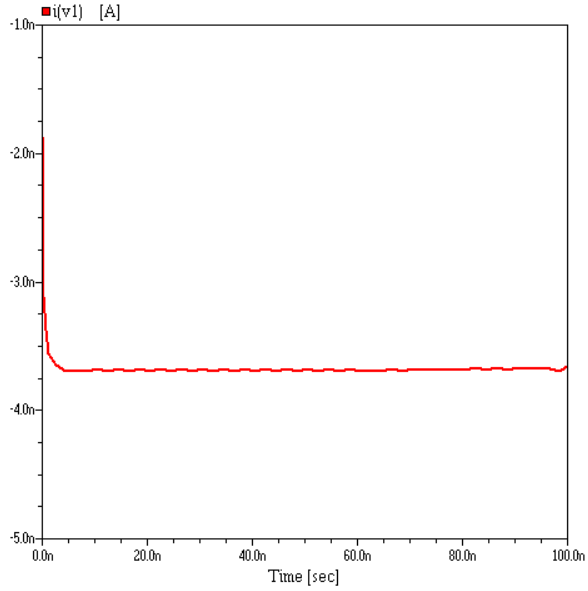
\includegraphics[width=0.3\linewidth]{aimSpice/plots/plotsTT/leak.png}
    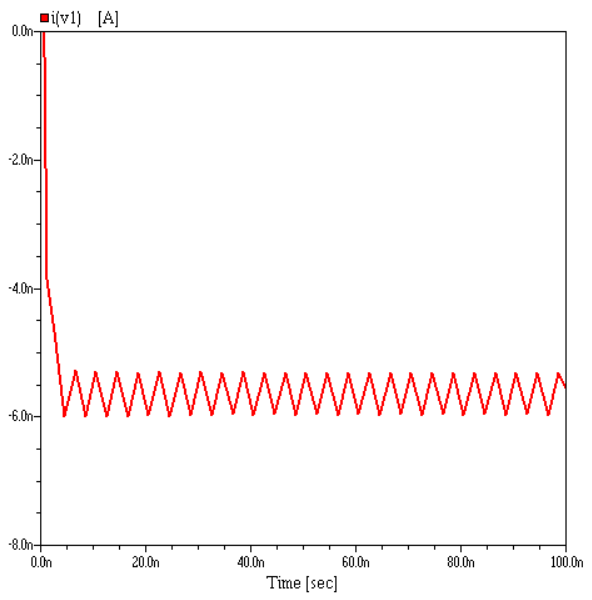
\includegraphics[width=0.3\linewidth]{aimSpice/plots/plotsFF/leak.png}
    \caption{Leakage currents at SS, TT and FF (from left to right).}
    \label{fig:04:leakage}
\end{figure}

\subsubsection{Read time}
The read times can be seen in \autoref{fig:04:read}. They are all shorter than 3ns, as was required in the project description.

\begin{figure}[H]
    \centering
    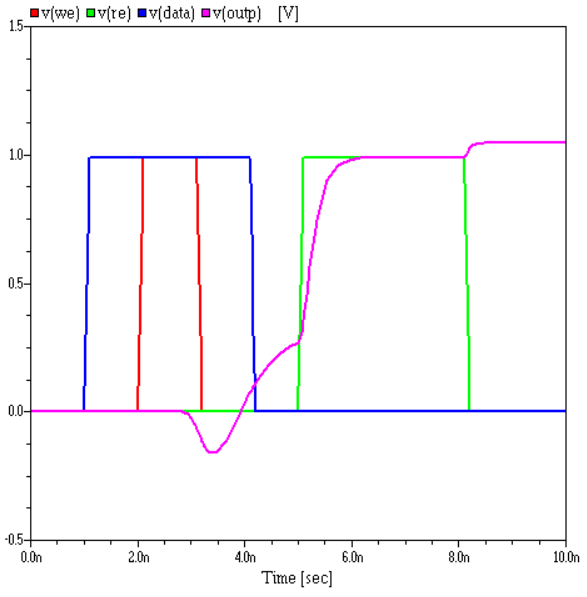
\includegraphics[width=0.3\linewidth]{aimSpice/plots/plotsSS/read.png}
    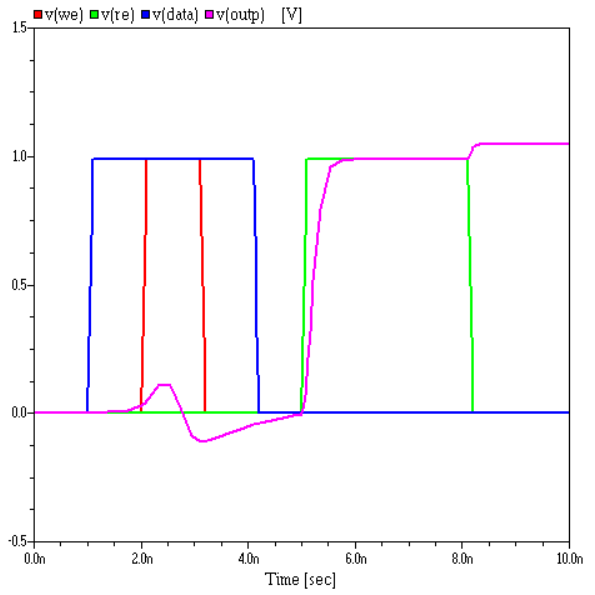
\includegraphics[width=0.3\linewidth]{aimSpice/plots/plotsTT/read.png}
    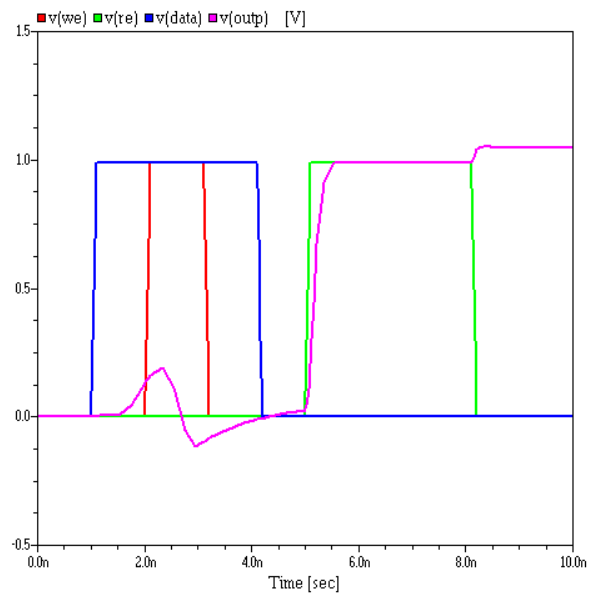
\includegraphics[width=0.3\linewidth]{aimSpice/plots/plotsFF/read.png}
    \caption{The read times to the bitcell at SS, TT and FF (from left to right) can be read as the time it takes v(outp) to reach v(re).}
    \label{fig:04:read}
\end{figure}

\subsubsection{Write time}
The write times can be seen in \autoref{fig:04:read}. They are also all shorter than 3ns, as was required in the project description.

\begin{figure}[H]
    \centering
    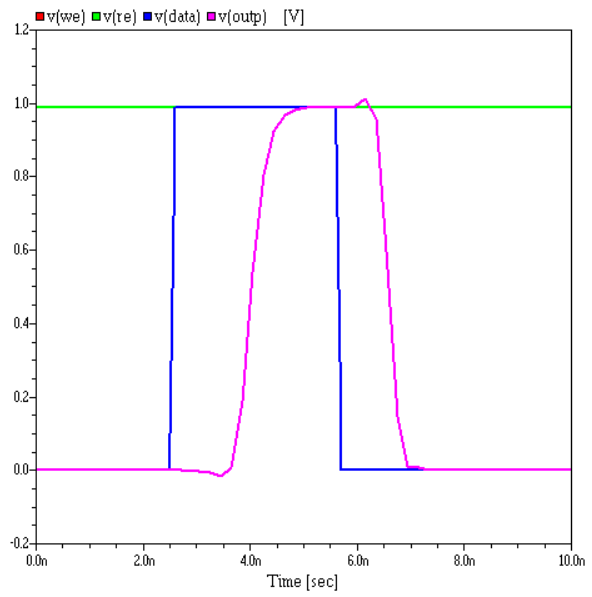
\includegraphics[width=0.3\linewidth]{aimSpice/plots/plotsSS/write.png}
    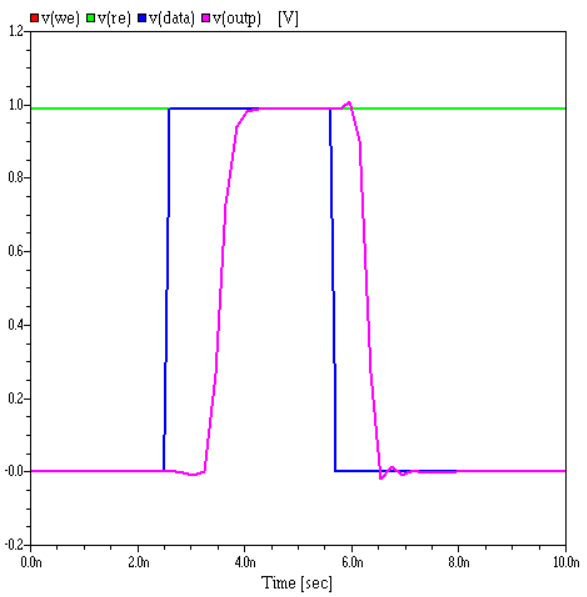
\includegraphics[width=0.3\linewidth]{aimSpice/plots/plotsTT/write.png}
    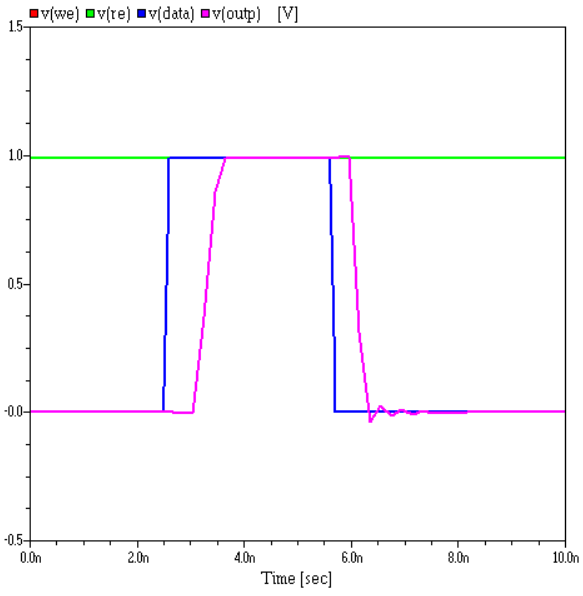
\includegraphics[width=0.3\linewidth]{aimSpice/plots/plotsFF/write.png}
    \caption{The write times to the bitcell at SS, TT and FF (from left to right) can be read as the time it takes v(outp) to reach v(data).}
    \label{fig:04:write}
\end{figure}

\subsubsection{Temperature Functionality}
The circuit is tested at three different temperatures (-20C, 27C, 50C) for five different circuit configurations (FF, FS, SF, SS, TT). The functionality tests behave well, and can be seen in \autoref{fig:04:func}. The test is comprised of writing and reading low, and then high, to the bitcell. 

\begin{figure}[H]
    \centering
    FF:
    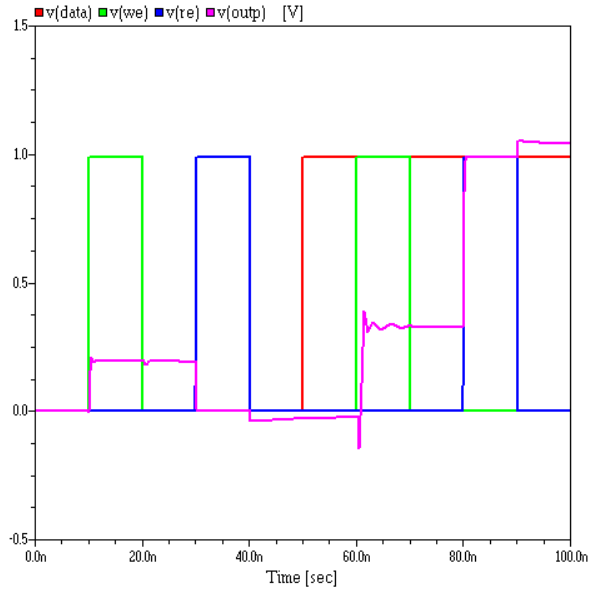
\includegraphics[width=0.24\linewidth]{aimSpice/plots/plotsFF/func-20c.png}
    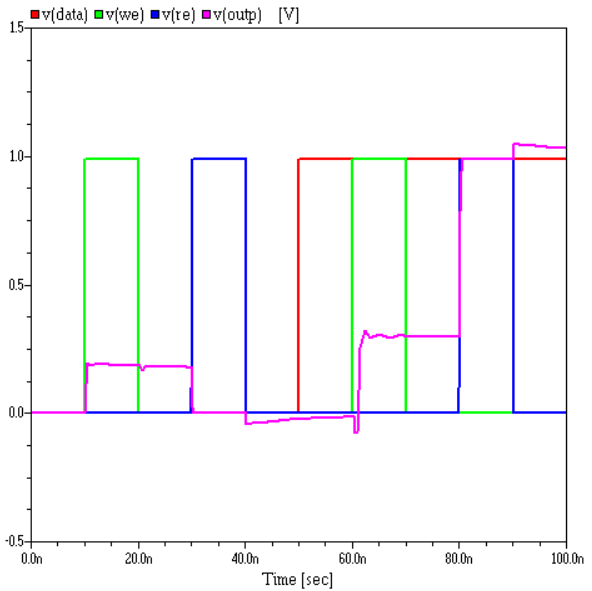
\includegraphics[width=0.24\linewidth]{aimSpice/plots/plotsFF/func27c.png}
    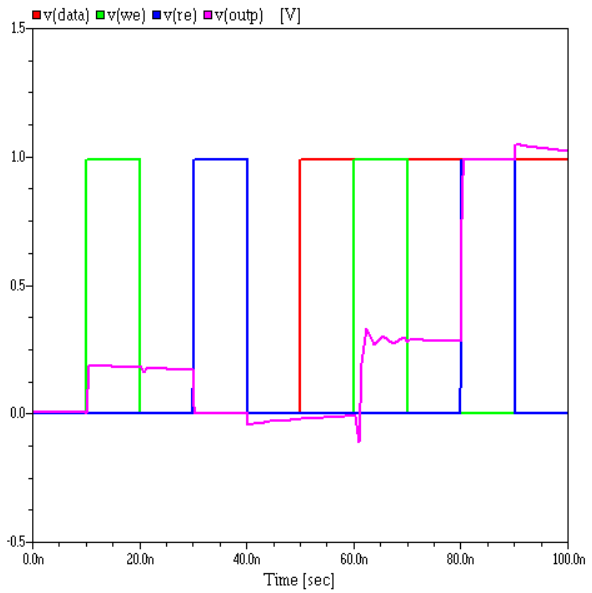
\includegraphics[width=0.24\linewidth]{aimSpice/plots/plotsFF/func50c.png}
    \newline
    FS:
    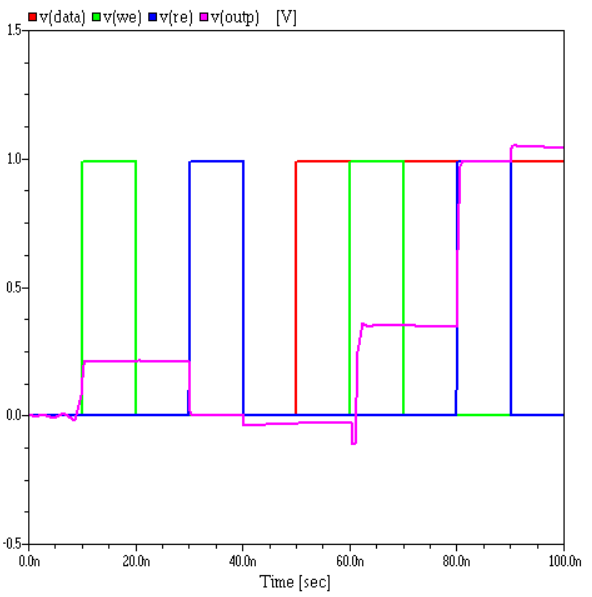
\includegraphics[width=0.24\linewidth]{aimSpice/plots/plotsFS/func-20c.png}
    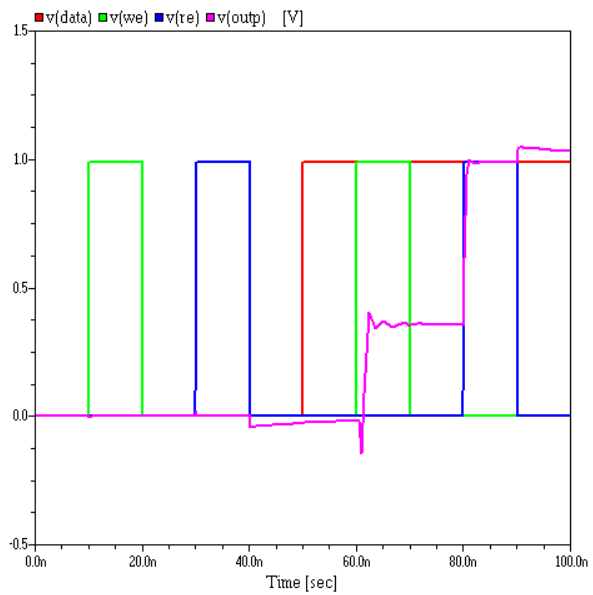
\includegraphics[width=0.24\linewidth]{aimSpice/plots/plotsFS/func27c.png}
    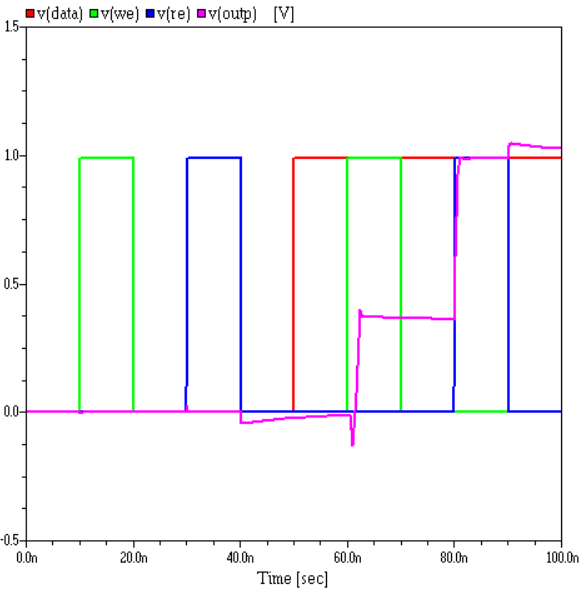
\includegraphics[width=0.24\linewidth]{aimSpice/plots/plotsFS/func50c.png}
    \newline
    SF:
    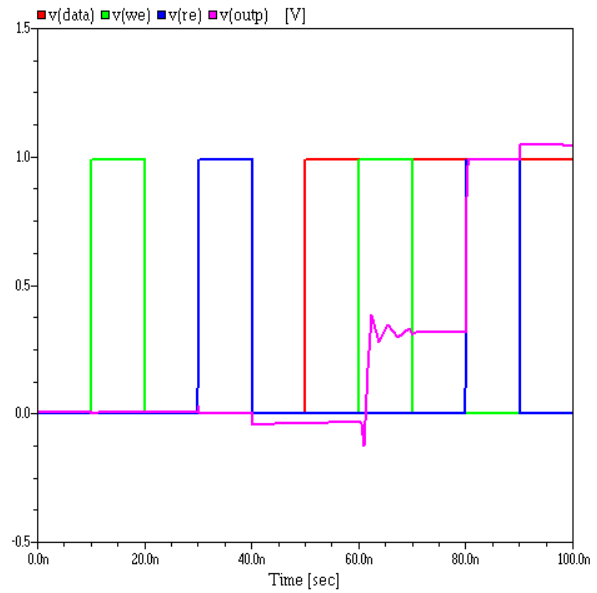
\includegraphics[width=0.24\linewidth]{aimSpice/plots/plotsSF/func-20c.png}
    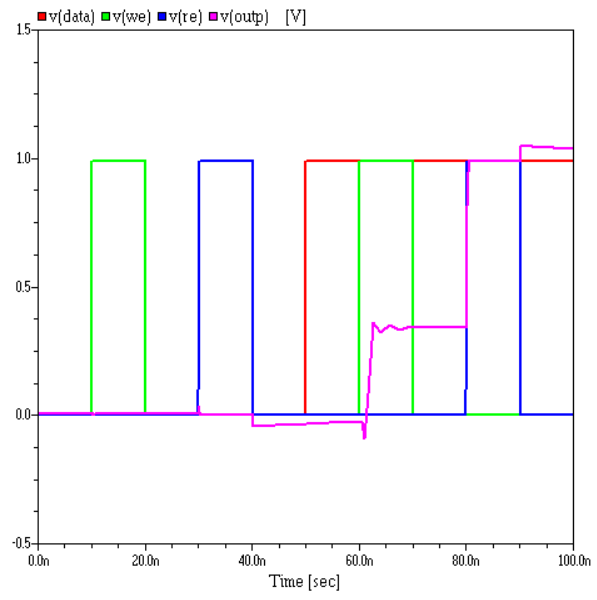
\includegraphics[width=0.24\linewidth]{aimSpice/plots/plotsSF/func27c.png}
    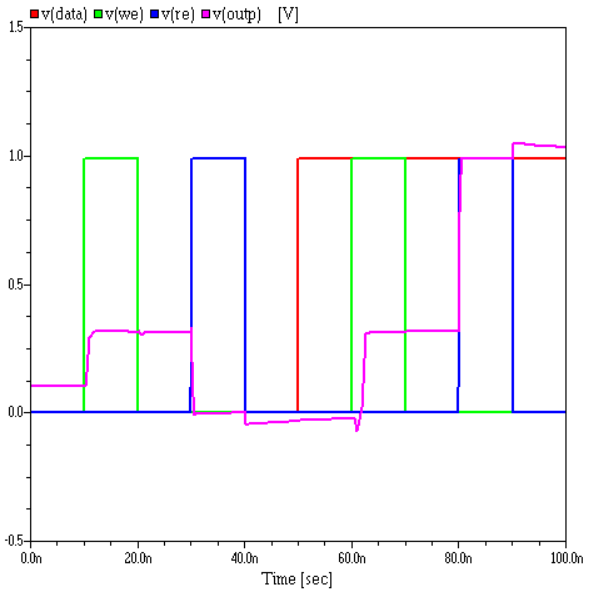
\includegraphics[width=0.24\linewidth]{aimSpice/plots/plotsSF/func50c.png}
    \newline
    SS:
    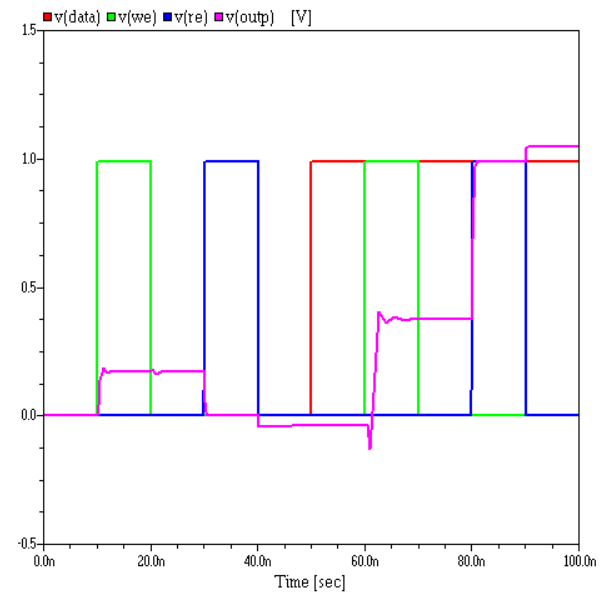
\includegraphics[width=0.24\linewidth]{aimSpice/plots/plotsSS/func-20c.png}
    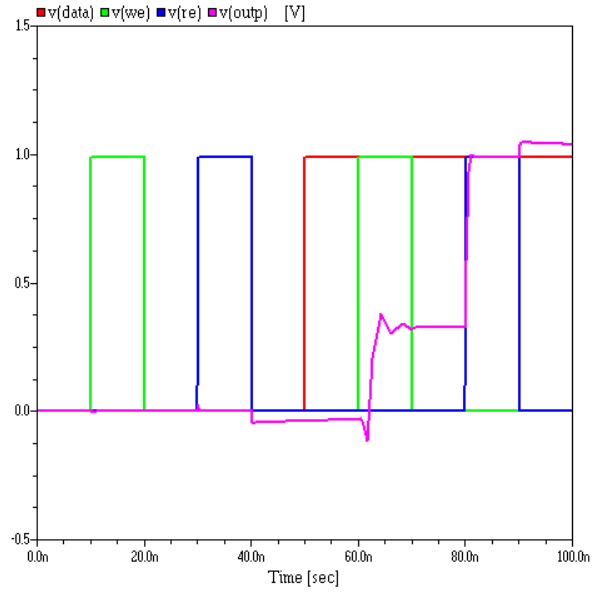
\includegraphics[width=0.24\linewidth]{aimSpice/plots/plotsSS/func27c.png}
    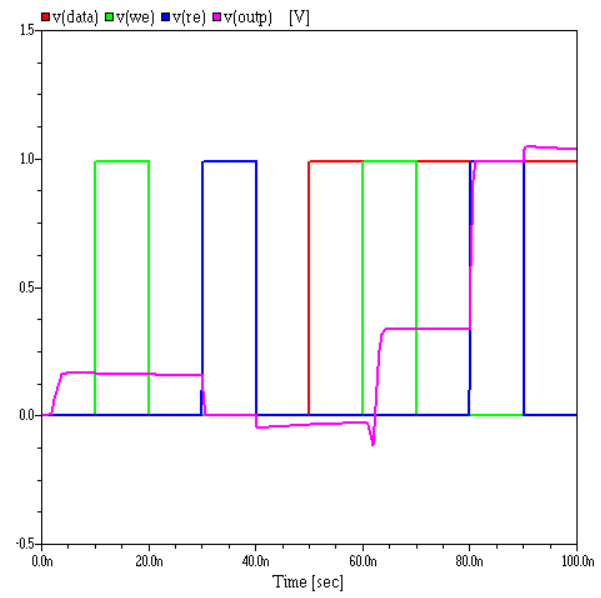
\includegraphics[width=0.24\linewidth]{aimSpice/plots/plotsSS/func50c.png}
    \newline
    TT:
    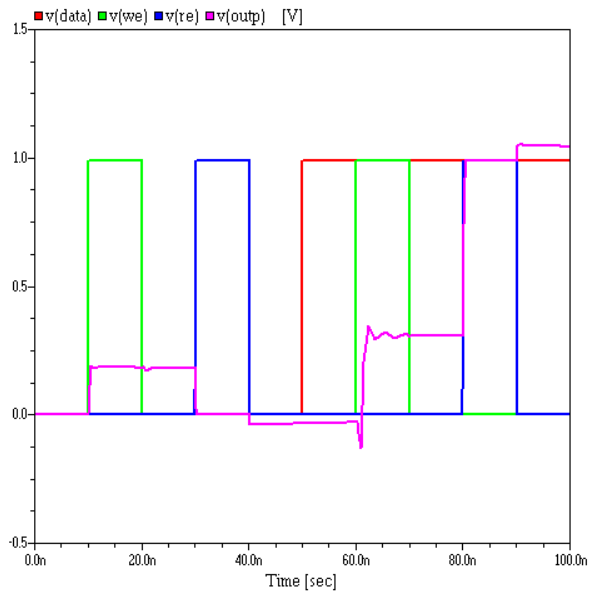
\includegraphics[width=0.24\linewidth]{aimSpice/plots/plotsTT/func-20c.png}
    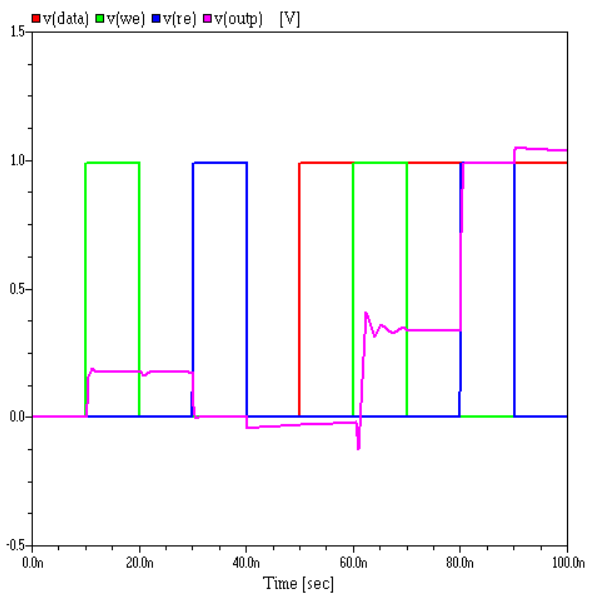
\includegraphics[width=0.24\linewidth]{aimSpice/plots/plotsTT/func27c.png}
    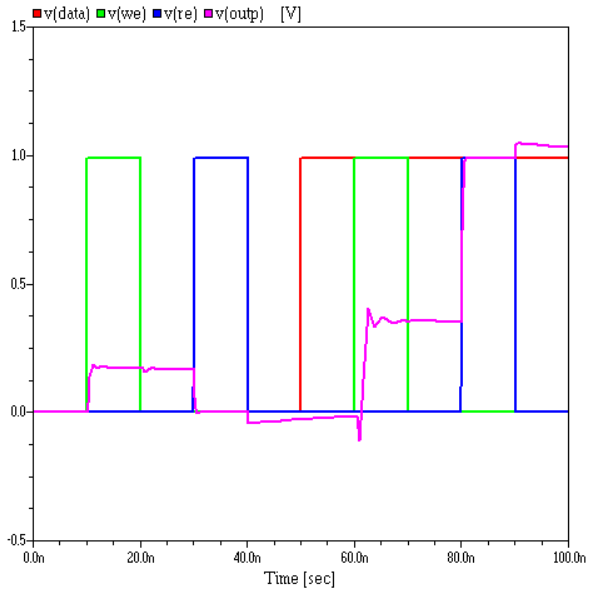
\includegraphics[width=0.24\linewidth]{aimSpice/plots/plotsTT/func50c.png}
    \newline
    
    \caption{The functionality tests of the bitcell. The left column is for -20\degree C, the middle column is for +27\degree C, and the right column is for +50\degree C. All tests meet the system requirements.}
    \label{fig:04:func}
\end{figure}

\subsection{Digital bitcell}    \label{sec:04:results:digital_bitcell}
The bitcell's behaviour is digitally simulated being given inputs and showing outputs according to what can be observed in \autoref{fig:04:bitcell_tb}.
\begin{figure}[H]
    \centering
    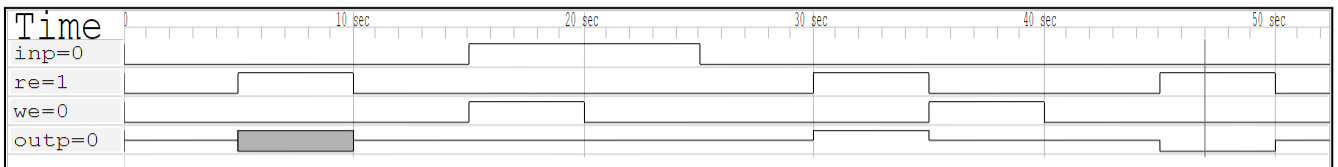
\includegraphics[width=0.9\linewidth]{LaTeX_2/Figures/bitcell_tb.png}
    \caption{Testbench of the bitcell}
    \label{fig:04:bitcell_tb}
\end{figure}
In the testbench we read the bitcell before any value has been set, expecting a undefined output. Then we write a logic high, read the logic high, write a logic low, and read that too. When RE is low, we expect to see a high-impedance value, $Z$, which is observed. REN is not shown in the figure, since it is trivial. The subsystem performed exactly as expected.

\subsection{Demux}
The demux' behaviour is digitally simulated being given inputs and showing outputs according to what can be observed in \autoref{fig:04:demux_tb}.

\begin{figure}[H]
    \centering
    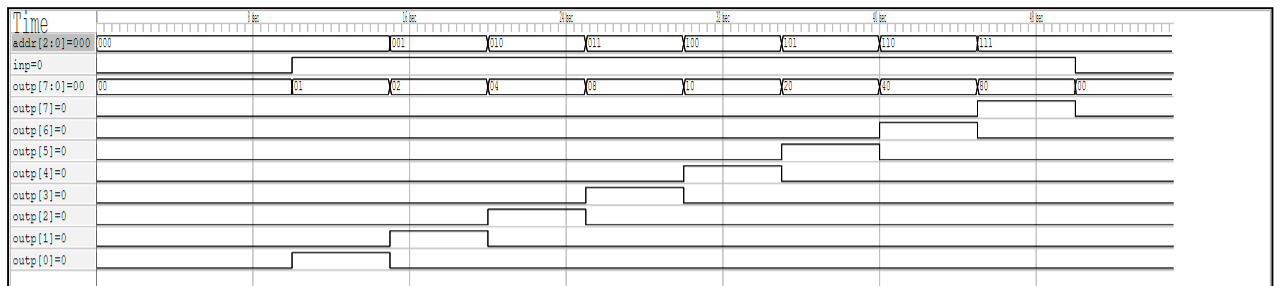
\includegraphics[width=0.8\linewidth]{LaTeX_2/Figures/demux1to8_tb.png}
    \caption{}
    \label{fig:04:demux_tb}
\end{figure}
In the testbench we cycle through all of the outputs, checking that each of them can be set high, and that all the other ones are low if that is the case. The subsystem performed exactly as expected.

\subsection{RAM}
The RAM subsystem's behaviour is digitally simulated being given inputs and showing outputs according to what can be observed in \autoref{fig:04:ram_tb}.
\begin{figure}[H]
    \centering
    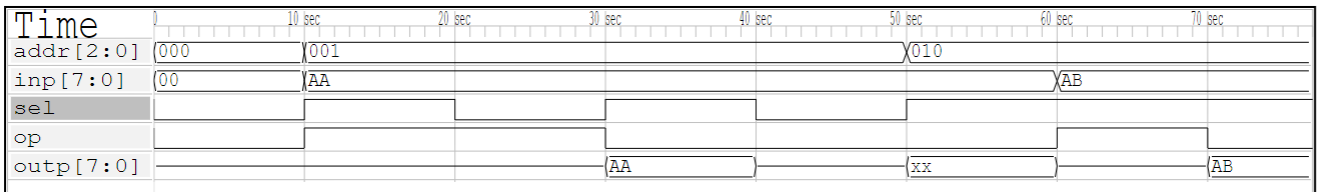
\includegraphics[width=0.9\linewidth]{LaTeX_2/Figures/ram_tb.png}
    \caption{Testbench of the RAM}
    \label{fig:04:ram_tb}
\end{figure}
In the testbench we write the 8-bit hex value $AA$ into address $001$, and read that value. Then, we go to address $010$ and read what is stored there, which should be undefined, $xx$, since nothing has been written to this address yet. We then write the hex value $AB$ to this address and read to observe that it has changed from $xx$ to $AB$. The subsystem performed exactly as expected.

\subsection{FSM}
The FSM subsystem's behaviour is digitally simulated being given inputs and showing outputs according to what can be observed in \autoref{fig:04:FSM_tb}.
\begin{figure}[H]
    \centering
    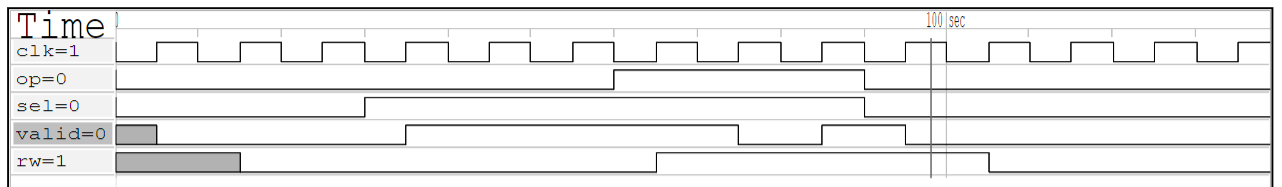
\includegraphics[width=0.9\linewidth]{LaTeX_2/Figures/FSM_tb.png}
    \caption{Testbench of the FSM}
    \label{fig:04:FSM_tb}
\end{figure}

In the testbench we check that the FSM can enter all of its four states: 

\begin{itemize}
    \item We start by waiting two clock cycles for it to settle into the \textit{IDLE} state. 
    \item Then we set \textit{sel} high, which causes the FSM to go into the \textit{READ} state on the next rising edge, which can be seen by the FSM's outputs. 
    \item After making sure the state is stable, we set \textit{op} high as well, causing the FSM to go into the \textit{WRITE} state. 
    \item Here it will go to the \textit{STABLE} state on the next clock cycle, no matter the input, but we keep the inputs as before to make sure it then goes back to \textit{WRITE} again. 
    \item Lastly, we observe the FSM going back to \textit{IDLE} when both inputs are low.
\end{itemize}
The FSM performed as expected.

\subsection{Complete memory module} \label{sec:04:results:complete_memory_module}
The behaviour of the complete memory module system, with the FSM subsystem controlling the inputs to the RAM subsystem, is digitally simulated being given inputs and showing outputs according to what can be observed in \autoref{fig:04:mem_system_tb}.
\begin{figure}[H]
    \centering
    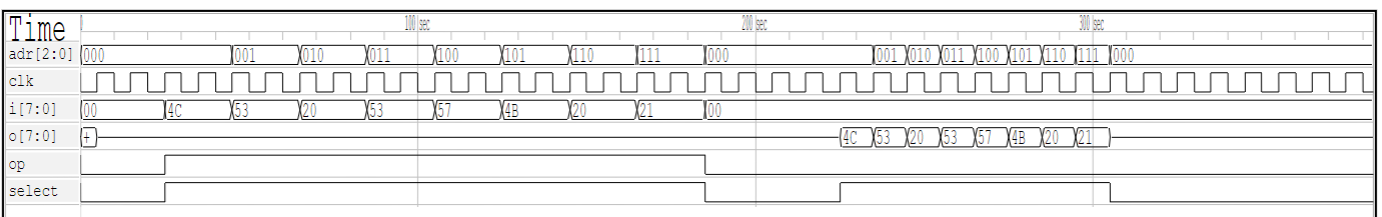
\includegraphics[width=0.9\linewidth]{LaTeX_2/Figures/mem_system_tb.png}
    \caption{Testbench of the complete memory module}
    \label{fig:04:mem_system_tb}
\end{figure}
In this testbench we write our names' initials into the memory module, and then read them. The ASCII symbols to store are \textit{"LS SWK !"}, which converted to hex is $[4C, 53, 20, 53, 57, 4B, 20, 21]$. Writing takes two clock cycles, since the FSM has to go into the \textit{STABLE} state between address switching, and reading takes one clock cycle. The completed system performed as expected.